\scanpage{31}
% paper watermark, sideways, first fragment clipped at the upper edge
{\centering \textsc{\unsure{Extr}\unsure{a}}\\
\textit{\unsure{Ma}\unsure{in|i|nn}}\par}
\figure{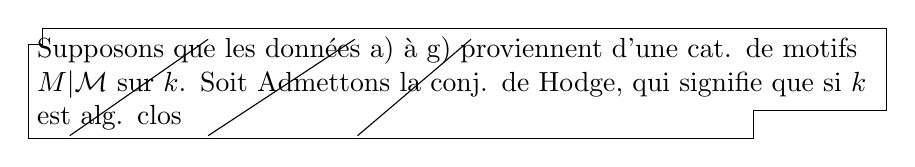
\begin{tikzpicture}[x=1cm,y=1cm]
\node[inner sep=3pt,text width=.88\linewidth,align=left] (oldblock) {\deleted{Supposons que les données a) à g) proviennent d'une cat. de motifs $\unsure{M|\mathcal M}$ sur $k$. \deleted{\unsure{Soit}} Admettons la conj. de Hodge, qui signifie que si $k$ est alg. clos}};
\draw ([xshift=5pt]oldblock.north west) -- (oldblock.north east) -- ([yshift=10pt]oldblock.south east) -- ([xshift=-48pt,yshift=10pt]oldblock.south east) -- ([xshift=-48pt]oldblock.south east) -- (oldblock.south west) -- ([yshift=-6pt]oldblock.north west) -- ([xshift=5pt,yshift=-6pt]oldblock.north west) -- cycle;
\draw ([xshift=15pt,yshift=1pt]oldblock.south west) -- ([xshift=65pt,yshift=-4pt]oldblock.north west);
\draw ([xshift=65pt,yshift=1pt]oldblock.south west) -- ([xshift=118pt,yshift=-4pt]oldblock.north west);
\draw ([xshift=119pt,yshift=1pt]oldblock.south west) -- ([xshift=160pt,yshift=-4pt]oldblock.north west);
\end{tikzpicture}}

Soit $V_{\mathbb Q},\ V_{\mathbb C}=\sum_{pq}V^{pq}$ une structure de Hodge, et soit $G$ son gpe de Mumford-Tate, donc $G_{\mathbb C}\subset\underline{\mathrm{Aut}}_{\mathbb C}(V)$. Soit $V_k\subsetV_{\mathbb C}$ une restriction des scalaires de $\mathbb C$ à $k\subset\mathbb C$, \deleted{\unsure{une}} \uline{compatible} avec la filtration naturelle de $V_{\mathbb C}$. Supposons que $(V_{\mathbb Q},\,V_{\mathbb C}=\sum V^{pq},\,V_k\subset V_{\mathbb C})$ provienne d'un motif sur \uuline{$k$}. \inserted{\deleted{Admettant}} \deleted{et admettons la conj. \unsure{de H.|de h}} \deleted{Alors}

Le gpe de Galois motivique de ce dernier, rel. à $T_{\mathrm{DR}}$, est \unsure{une|un} \deleted{forme} \inserted{groupe} $G'$ \unsure{déf}/$k$, \deleted{de $G_{\mathbb C}$,} et en vertu de \uline{conj. de Hodge} on doit avoir $G'_{\mathbb C}\unsure{=|\subset}G^\circ_{\mathbb C}$. \deleted{(\unsure{d'après} \illegible{2})} En d'autres termes, il faut que $G^\circ_{\mathbb C}$ soit ``définissable sur $k$ via $V_k\subset V_{\mathbb C}$'' ; c'est une condition très ; fort non triviale ! Lorsque $k$ est alg. clos, il faudra \deleted{\unsure{en}} $G'_{\mathbb C}=G_{\mathbb C}$, ce qu'on peut exprimer en disant que $\unsure{\forall|H}$ \deleted{invariant} élément d'un ${\bigotimes}_{\mathbb Q}^{\unsure{n|m}}(V'\otimes_{\mathbb Q}V)$ invariant sous $G$ (i.e. de bidegré $0$) est nécessairement dans $\bigotimes_{\unsure{k'|\bar k}}^{\unsure{n|m}}(V'_{\unsure{k'|\bar k}}\otimes_{\bar k}V_{\unsure{k'|K'}})$\unsure{!} ; si $k$ général, il faut \deleted{remplacer $k$ par une extension} \inserted{donc $\exists$ extension finie $k'$ de $k$,} ayant la vertu précédente. Ce sont encore des conditions très restrictives sur la structure envisagée. Elles ne sont certainement pas suffisantes (faire $k=\mathbb Q$, $V_k=V_{\mathbb Q}$, ce n'est en général pas possible
\figure{\begin{tikzpicture}[x=1pt,y=1pt]
\draw[dash pattern=on 8pt off 4pt] (0,0) -- (49,0);
\draw (55,6) -- (60,6) -- (61,0) -- (55,0);
\end{tikzpicture}}
% paper watermark, sideways, second fragment clipped at the lower edge
{\centering \textsc{\unsure{Strong}}\\
\textit{\unsure{uy|ny|y} \unsure{1808}}\par}
% archive sheet number: 30
